\documentclass[a4paper]{article}
\usepackage{authblk}
\usepackage[backend=bibtex]{biblatex}
\usepackage{hyperref}
\usepackage{txfonts}
\usepackage{titling}
\usepackage{graphicx}
\usepackage{subcaption}
\usepackage[a4paper, margin={2.5cm, 1.7cm}]{geometry}
\usepackage{mwe}
\usepackage{filecontents}
\usepackage{changes}
\usepackage{lipsum}% <- For dummy text
%\definechangesauthor[name={Heide}, color=blue]{Heide}
%\definechangesauthor[name={Jonas}, color=magenta]{Jonas}
%\setremarkmarkup{(#2)}

\bibliography{database.bib}

\begin{document}
\title{Fast processing of JUNGFRAU data with the Alpaka library}
\author{Jonas Schenke$^{1,2}$, 
Florian Warg$^{1,2}$, 
Anna Bergamaschi$^3$,
Martin Br\"uckner$^3$,\\
Michael Bussmann$^1$,
Carlos Lopez-Cuenca$^3$,
Aldo Mozzanica$^3$,\\
Sophie Redford$^3$,
Bernd Schmitt$^3$,
Heide Mei{\ss}ner}

\affil[1]{Helmholtz-Zentrum Dresden -- Rossendorf, Bautzner Landstra{\ss}e 400, 01328 Dresden, Germany}
\affil[2]{Technische Universit\"at Dresden, 01069 Dresden, Germany}
\affil[3]{Paul Scherrer Institut, 5232 Villigen-PSI,  Switzerland}



\date{}

\renewcommand\Affilfont{\itshape}



\maketitle
{\bf Abstract}\\
Highly segmented photon detectors play a crucial role at synchrotron and X-ray free electron laser facilities, detecting the photons scattered from targets of interest. These measurements allow the determination of biological and inorganic structures and processes, leading to an advanced understanding of life and material sciences and enabling improvements and discoveries in pharmaceutical and engineering industries. However, as targets become ever-more challenging and photon fluxes intensify, detector frame rates increase and the generated data streams risk becoming overwhelming. Here we demonstrate one solution, exploiting the highly parallelisable nature of data from the JUNGFRAU charge integrating photon detector and processing using the Alpaka library. We find that... To date, no other solution was able to process JUNGFRAU data at this throughput(?). Our results demonstrate that parallel processing, for example in a GPU, is a valuable tool in the treatment of photon detector data. Advantages of this method include online data correction aiding storage efficiency by allowing raw data to be immediately discarded and enabling fast feedback to users for whom time and target resources are at a premium. We see this as an important step in the development of a chain of specialised hardware and software tools necessary to operate charge integrating photon detectors at high frame rates.

{\bf Keywords:} Photon pixel detector, fast data processing, GPU programming, Alpaka...



\section{Introduction}

Data rates and volumes at photon science facilities are increasing due to many technological advancements, including higher beam intensities, robotic or serial sample delivery systems, and photon detectors capable of ever increasing frame rates. Charge integrating detectors compound the issue, as the raw detector output must be processed before the number of photons detected is retrieved. This requires advanced methods for fast, online data processing without which data volumes threaten becoming a limiting factor, quickly filling storage capacity, overwhelming computing processing power and slowing feedback to users.

The JUNGFRAU detector is one such charge integrating photon detector~\cite{Mozzanica_2016}, which has been designed for SwissFEL, the free electron laser at the Paul Scherrer Institut in Switzerland~\cite{SwissFEL}. Two 16 Mpixel JUNGFRAU detectors were installed at SwissFEL in 2018 and are now operational~\cite{JFapplications}. Due to the repetition rate and pulsed illumination of SwissFEL, the detectors are operated continuously with short ($10\;\mu\mathrm{s}$) integration time and at a frame rate of 100 Hz, meaning that each 16 Mpixel detector generates a reasonable data rate of 3.2 GB/s. 

However, JUNGFRAU has also proved advantageous under challenging conditions at synchrotrons~\cite{Leonarski_2018} where the illumination is continuous, requiring a full duty cycle from the detector and hence much higher frame rates. Recent experimental setups have included a one Mpixel detector operated continuously at 1.1 kHz (2.3 GB/s) with online visualisation but slow offline data treatment~\cite{Leonarski_2018} and a four Mpixel detector operated at 1.1 kHz (9.2 GB/s) for short periods of time ($<200$ s) without visualisation but with fast data processing straight after acquisition (Japan, no ref yet). Our goal is to operate a 16 Mpixel detector continuously at 2.2 kHz, successfully receiving the raw data at 74 GB/s, providing an online visualisation, processing it online to convert the raw data into number of photons per pixel, and saving to disk. This necessitates specialised capability for receiving, processing and file writing, motivating this work.

The increasing data rates during FEL experiments require dedicated detectors as well as advanced methods for fast data processing.
At PSI, the Jungfrau detector (\cite{JFapplications}, \cite{JFcalibration}, \cite{JFoperation}, \cite{Mozzanica_2016}) was developed which is capable due to a gain switching scheme to register single photons as well as photon bunches in a charge integration mode. A conversion of the detector data to the energy and the number of registered photons already during data acquisition is beneficial for the analysis of the measurement and furthermore for the reduction of storage space. This online data conversion algorithm has to correct each pixel value using the gain maps and the continuously updated pedestal maps following a lab-based calibration  procedure~\cite{JFcalibration}. The summation of a couple of frames and the cluster identification in the data maps further reduce the amount of data. The different modules of one detector system can be processed fully parallel, however, the data conversion itself is not data parallel. Therefore, and due to the need for an advanced parallel implementation which is independent of the computing hardware, an Alpaka \cite{Matthes17} version was written and its performance was tested.\\

\textcolor{blue}{TODO: Related work}\\
\textcolor{magenta}{
common pre-processing steps:
\begin{itemize}
	\item offset correction \& flat field correction [DSSC \cite{moch2014calibration}, JF \cite{JFcalibration}, EIGER\cite{tinti2018electron} / \cite{dinapoli2013eiger}, MOENCH \cite{cartier2016micrometer}, [MEDIPIX3RX \cite{ballabriga2013medipix3rx}]]
	\item gain correction [DSSC \cite{moch2014calibration}, EIGER \cite{tinti2018electron} / \cite{dinapoli2013eiger}, MOENCH \cite{cartier2016micrometer}]
	\item dynamic gain switching [AGIPD \cite{allahgholi2015agipd}, GOTTHARD \cite{mozzanica2012gotthard}, JF \cite{JFcalibration}, [MEDIPIX3RX \cite{ballabriga2013medipix3rx}]
	\item pixel sorting (on FPGA)[AGPID \cite{becker2013high}]
	\item discard uninteresting events (in readeout circuit)[DSSC \cite{erdinger2012dssc}]
	\item photon counting [MEDIPIX3RX \cite{ballabriga2013medipix3rx}]
	\item charge summing / interpolation (to counter charge sharing; on ASIC)[MEDIPIX3RX \cite{ballabriga2013medipix3rx}]
	\item cluster finder [MOENCH \cite{cartier2016micrometer}]
	\item sub pixel interpolation [MOENCH \cite{cartier2016micrometer}]
\end{itemize}
detector data processing libraries (with pre-processing stage):
\begin{itemize}
	\item Karabo \cite{fangohr2018data}
	\begin{itemize}
		\item developed to support experiments at the European XFEL
		\item written in C++ and Python
		\item pipelined design
		\item supports offline and online operation and an additional rapid-feedback mode
		\item can utilize multiple nodes
		\item also implements file IO and a GUI
		\item extensible through Karabo-Bridge
		\item has OnDA interface
		\item supports Jupytier notebook
	\end{itemize}
	\item Hummingbird \cite{daurer2016hummingbird}
	\begin{itemize}
		\item optimized for real-time usage
		\item implemented in Python
		\item main purpose: analysis of diffraction data at LCLS
		\item achieves rates above 100 Hz
		\item contains a GUI and supports multiple file streams at once
		\item can utilize multiple computing nodes
		\item can read data generated by psana
	\end{itemize}
	\item OnDA \cite{mariani2016onda}
	\begin{itemize}
		\item supports online \& offline operation
		\item can utilize multiple computing nodes (via ZeroMQ and MPI)
		\item master/worker architecture
		\item one program instance per core
		\item designed to give fast online feedback
		\item main objective: real-time monitoring of X-ray imaging experiments
		\item easily adaptable
		\item contains a GUI
		\item implemented in Python
		\item can utilize a psana back end
	\end{itemize}
	\item psana \cite{damiani2016linac}
	\begin{itemize}
		\item = Photon Science ANAlysis
		\item similar functionality to pyana (which is written entirely in Python), but implemented mostly in C++ with a Python interface
		\item used to analyze data produced by SLAC National Laboratory
		\item can utilize multiple compute nodes (via MPI)
		\item supports online \& offline operation
		\item contains detector calibration algorithms (e.g. pedestal calibration, bad-pixel determination, etc.) and GUI front end
		\item designed to give fast online feedback
	\end{itemize}
	\item Cheetah \cite{barty2014cheetah}
	\begin{itemize}
		\item mode for XFEL applications
		\item offline \& online processing
		\item evaluates data quality metrics (e.g. number of Bragg peaks etc.)
		\item retain only frames with high likelihood of being usable
		\item --> main task: data reduction
		\item additional pre-processing
		\item also has a GUI
		\item implemented in C++
	\end{itemize}
	\item CASS \cite{foucar2012cass}
	\begin{itemize}
		\item evaluate data acquired using the CFEL ASG Multi Purpose instrument (CAMP), specifically data collected at FLASH and the European XFEL
		\item supports multiple detectors in online and offline scenarios
		\item implemented in C++ with a Qt front end
		\item consists of input ringbuffer and processing modules (which do pre- \& post-processing)
		\item GUI implemented in two additional programs: joCASSView (plots data) \& luCASSView (interactive)
		\item GUIs communicate with computation nodes via TCP/IP
	\end{itemize}
	\item XDS \cite{kabsch2010xds}
	\begin{itemize}
		\item in development since 1988
		\item mainly deals with crystallography
		\item also does pre-processing steps
		\item no real-time/on-line capability
	\end{itemize}
\end{itemize}
initialized data further used e.g. in crystallography \cite{kabsch2010integration} \cite{white2012crystfel} \cite{grosse2002computational}}\\

In section~\ref{subsec:det}, we review the design of Jungfrau detectors, followed by the description of the dedicated data conversion algorithm~\ref{subsec:alg}, its hardware-independent implementation~\ref{subsec:alpaka} and benchmark tests in~\ref{subsec:benchmark}. The achieved results and conclusions are presented in sections~\ref{sec:results} and \ref{sec:conclusions}. 


\section{Methods}
\subsection{JUNGFRAU detector description (PSI)}
\label{subsec:det}
JUNGFRAU is a hybrid photon detector consisting of a $320\;\mu\mathrm{m}$ thick silicon sensor in which photons are absorbed and converted into an electrical signal, and an Application Specific Integrated Circuit (ASIC) chip in which the signal generated by the photons in the silicon is processed. Both sensor and ASIC layers are pixelated with $75\;\mu\mathrm{m}$ pitch, to provide two dimensional information of the position of the incident photons.

The JUNGFRAU ASIC is realised with UMC 110 nm CMOS technology and operates in the `charge integrating' mode, meaning that the signal received by the ASIC within a well-defined, configurable time window (an exposure) is integrated and amplified~\cite{Mozzanica_2016}. Charge integrating detectors typically suffer from either a low dynamic range or poor resolution in the single photon regime. JUNGFRAU achieves both high dynamic range and single photon resolution by employing a gain switching technique, whereby the amplification factor of the initial photon-induced signal is dependent on the size of the signal itself. The gain switching happens automatically and independently per pixel and per exposure. The gain factor employed by each pixel (high, medium or low) in each exposure is encoded in a 2-bit output.

Each sensor has the dimensions of $1030\times514$ pixels, resulting in an active area of $7.7\times3.8$ cm$^2$. Eight $256 \times 256$ pixel ASICs are bump-bonded to each sensor in $4\times2$ arrangement to achieve an electrical connection in every pixel.  Between the ASICs are two rows or columns of double-sized pixels, ensuring no gaps or loss of sensitivity. The eight ASICs are glued to a high density interconnect (HDI) and electrically connected with wire-bonds along the two long sides. Additional wire-bonds to the sensor provide the high voltage to bias the sensor, crucial for detecting the charge generated there by the absorbed photons. A readout board connects to the back of the HDI to collect the signals processed by the eight ASICs. Four 14-bit ADCs convert the incoming analogue signal to digital samples. An FPGA arranges this 14-bit signal information from each pixel together with the 2-bit gain information of each pixel into a 1 MB image (a frame) of each exposure. This is output as UDP packets through two 10 Gb optical fibres.

This single detector module can either operate alone, or can be tiled together with other detector modules to form part of a larger detector system, with typical sizes ranging from 1 Mpixel (two modules) to 16 Mpixels (32 modules). Figure~\ref{fig:jfdetector} shows the front and back of a 4 Mpixel (8 module) detector. Each module retains its individual control (Ethernet), data (10 Gb optical fibres) and power connections. The only inter-module connection is a flat-ribbon cable used for triggering purposes. Data rates thus scale linearly with the number of modules.

While sending the UDP packets in parallel with 2$\times$10~Gb/s per module is less challenging, receiving them in one or a few spots for further processing is more complex. Implementing this on a standard hardware with a non-optimised Linux system easily results in packet loss due to CPU and memory bandwidth limitations. Several avenues to resolve this issue are under development. Offloading the CPU can be achieved on a software level by bypassing the network stack, which avoids several memory copies. Another option is to offload the full receiving process into an FPGA, which receives the UDP packets with it's 100~Gb/s interface, reassembles full images and sends them over PCIe directly into host via DMA or GPU memory over GPUDirect. This goes beyond the scope of the current work, which focuses on processing the successfully received JUNGFRAU data.

\begin{figure}[h!]
\centering
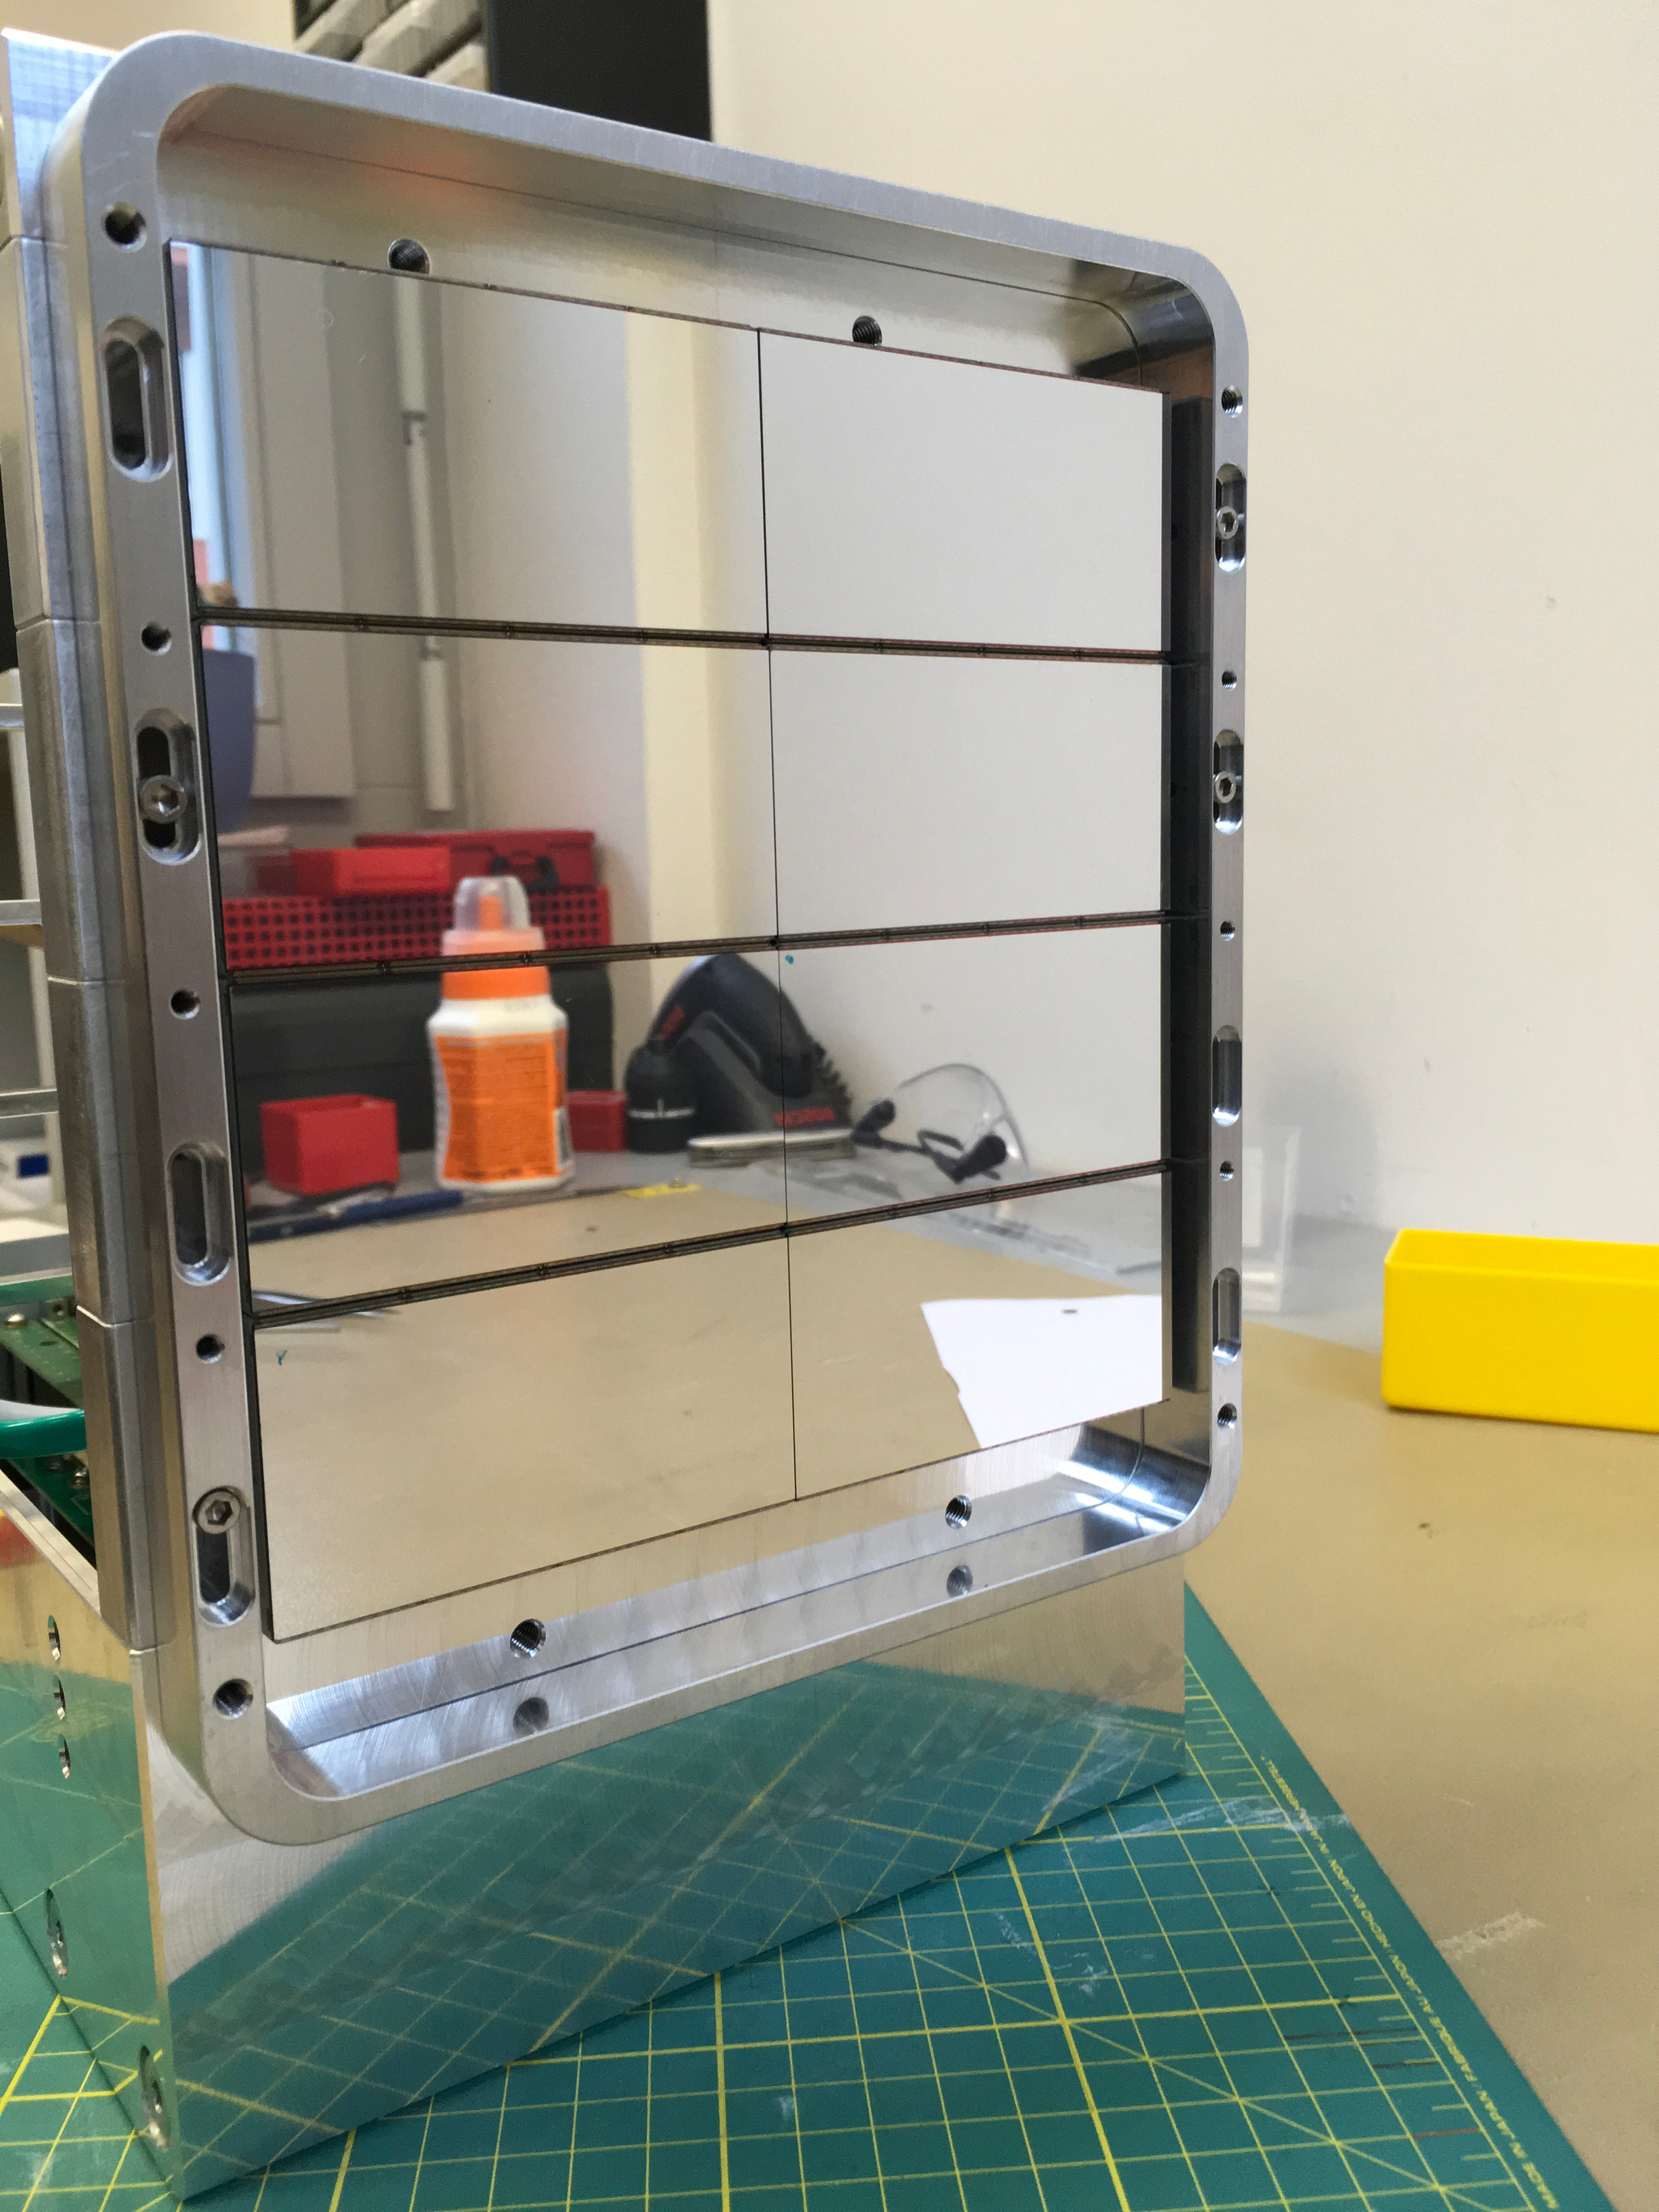
\includegraphics[width=0.30\textwidth]{jungfraudetector.jpg}
\hfill
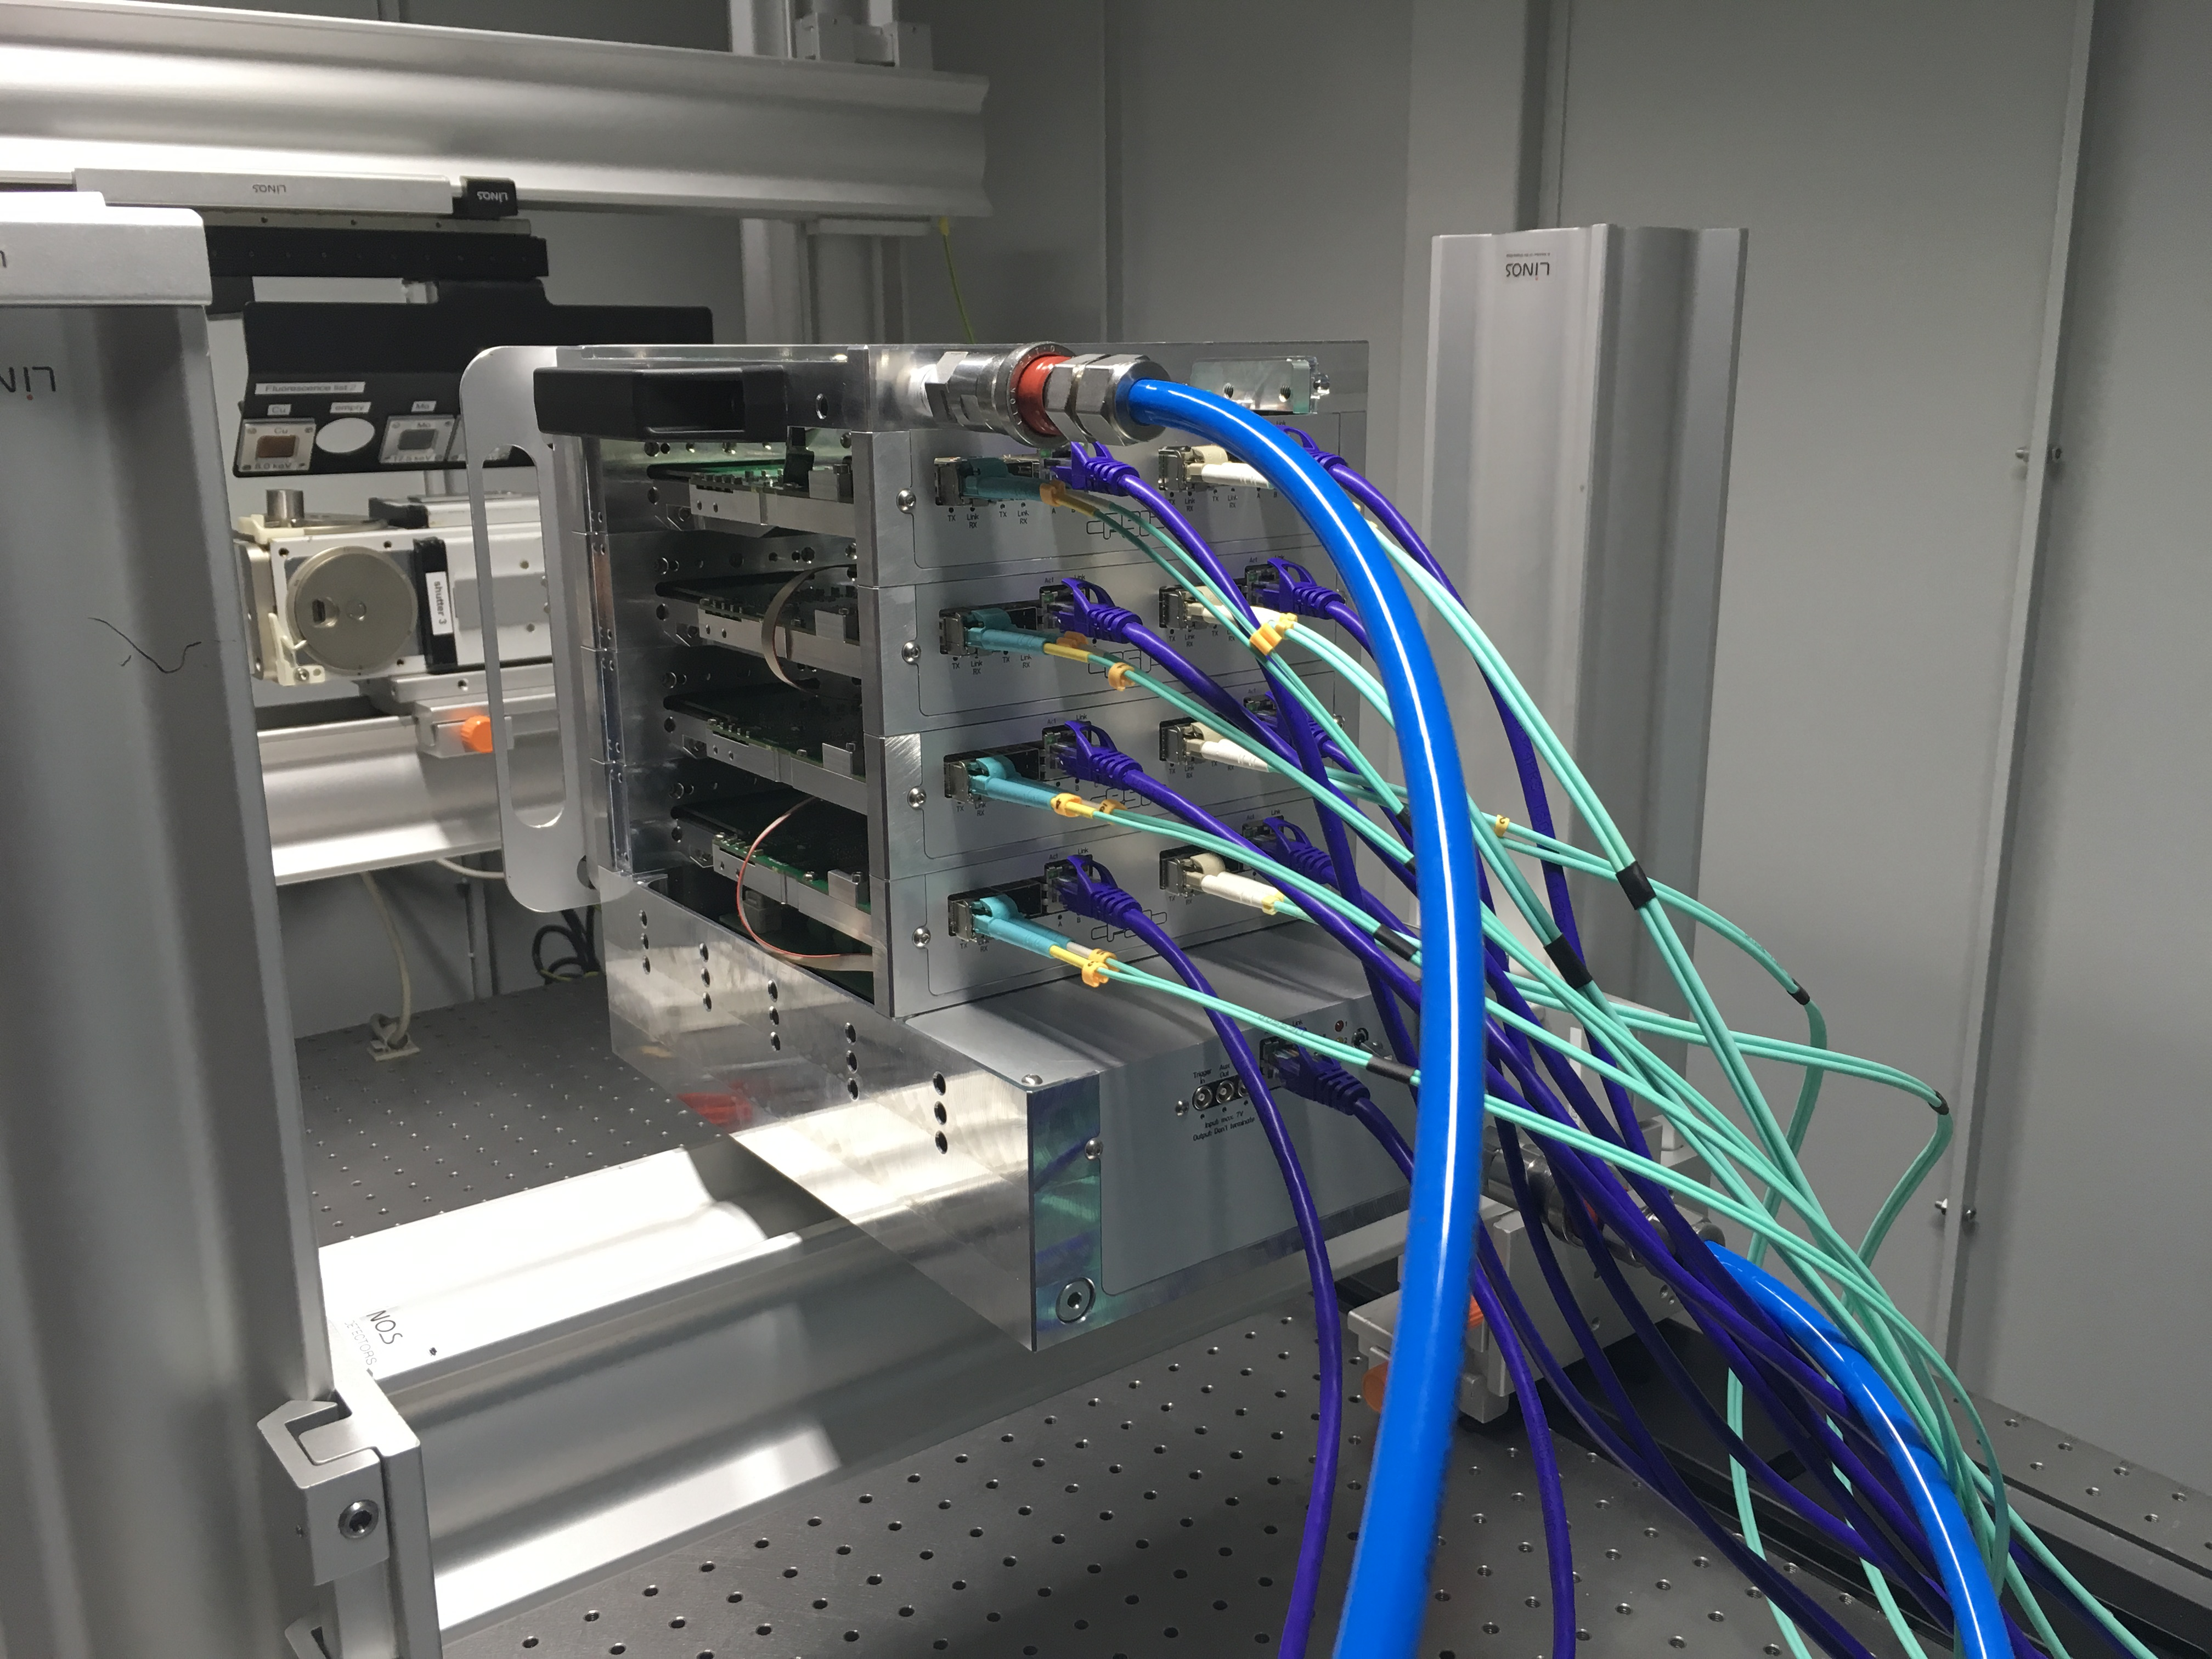
\includegraphics[width=0.50\textwidth]{JF4M_back.jpg}
\caption{A 4 Mpixel JUNGFRAU detector shown from the front (left) and back (right). Photons impinge on the eight mirrored sensor surfaces, which are tiled to ensure minimal dead area. The readout boards plug into the back of the modules. Each has its own Ethernet (purple cables) and optical fibre (green cables). Water cooling (blue pipes) and power (black cable) are provided in common. A flat ribbon cable, visible on the left, connects to all readout boards for triggering purposes.}
\label{fig:jfdetector}
\end{figure}


\subsection{Raw data treatment (PSI)}

To retrieve the information of how much energy, and in monochromatic situations, how many photons were detected in each pixel in each frame, a series of corrections must be applied to the raw 16-bit output of each pixel.

\subsubsection{Pedestal correction and tracking}
As any charge integrating detector, the JUNGFRAU detects some current in every pixel during every exposure, even if no photons were absorbed. This dark current or `pedestal' is individual to each pixel, and is strongly dependent on the configuration of the detector, for instance the exposure time, and on environmental factors such as temperature. It is therefore measured by acquiring a series of dark frames before each measurement with photons. To measure the pedestals in medium and low gain, the detector is forced to switch gain during the dark frames. The ADC values recorded in the dark frames in high, medium and low gain are averaged to give a per-pixel, per-gain pedestal. A rolling average is preferred [ref cook], both to avoid committing long arrays of data to memory, and to place higher importance on more recent exposures.

In the case of steady operation at XFELs, with a short integration time and the detector at room temperature, recording the pedestals every few hours is sufficient. However in the case of operation at synchrotrons, with a long integration time and the detector chilled to $\sim{-10}^{\circ}C$, the pedestals are much more sensitive~\cite{JFoperation}. They must be recorded before every measurement with photons, and moreover, must be tracked through the measurement. This is achieved by filtering the recorded exposures, and updating the pedestal measurement of a particular pixel if the frame recorded a value within $\pm2\sigma$ of the existing pedestal. This avoids exposures containing photon signals (typically $>10\sigma$ from the noise) from biasing the pedestal.

\subsubsection{Gain correction}
The pedestal-corrected ADC samples are translated into energies, so taking into account the amplification of the original signal by the ASIC. The amplification factors are calculated per pixel and per gain in a dedicated laboratory based procedure during the commissioning of the detector~\cite{JFcalibration}. Once the energy detected per pixel has been retrieved, in monochromatic situations this can be converted to a number of photons by normalising by the energy of the incident radiation, as shown in the following equation:
\begin{equation}
    N_{\gamma} = \frac{\mathrm{ADC\;output\;[ADU]} - \mathrm{pedestal\;[ADU]}}{\mathrm{gain\;[ADU/keV]} \times E_{\gamma} \mathrm{[keV]}}
\end{equation}
where $N_{\gamma}$ is the number of photons detected, $E_{\gamma}$ is the photon energy, and the pedestal and gain corrections are pixel dependent.

\subsubsection{Pixel mask}
A pixel mask can be defined using information from the calibration procedure and the pedestal calculation. Pixels can be non-responsive, or respond badly, for a number of reasons, including a chip level defect, bump bonding defect, wire-bond column defect or high leakage current. A pixel which could not be calibrated for any of these reasons, or could not have an accurate pedestal calculated, is masked in the later processing.

\subsubsection{Frame summation}
Depending on the application, further processing may be necessary. For macro-molecular crystallography, groups of subsequent frames (in our experience from 2 to 100 frames) can be summed together before saving~\cite{Leonarski_2018}. Depending on the rotation speed of the sample, this can improve later analysis to determine crystal structure. It also acts as an effective compression of the data.

\subsubsection{Pixel clustering}
In the case of soft X-rays at low incoming flux, pixels may be clustered to draw additional positioning information from the data. Description needed~\cite{Cartier_2015}.


\subsection{Data processing algorithm (PSI)}
\label{subsec:alg}
The following enumerates the typical data acquisition and processing steps for a single measurement with photons in a synchrotron environment, which is the most challenging in terms of data rate and which requires pedestal tracking.
\begin{enumerate}
\item acquisition of 1000 dark frames in forced switching to medium gain. The medium gain pedestal is calculated and pixels not in medium gain are added to the pixel mask.
\item acquisition of 1000 dark frames in forced switching to low gain. The low gain pedestal is calculated and pixels not in low gain are added to the pixel mask.
\item acquisition of at least 1000 dark frames in gain switching mode. Using the first 1000 frames, the high gain pedestal is calculated and pixels not in high gain are added to the pixel mask. At 1000 frames, pixels with larger than normal noise (pedestal RMS) are also added to the pixel mask and the noise level per pixel in high gain is taken as the pedestal tracking threshold. After 1000 frames, the high gain pedestal is tracked and the detector and software is `ready and waiting for photons'.
\item without stopping and restarting the detector, the beamline shutter opens and frames with photons are acquired in gain switching mode. Frames must be converted to number of photons per pixel. High gain pedestals are tracked. Frames can be optionally summed or clustered before being saved.
\end{enumerate}
Whether online or offline, whether implemented in CPU, GPU, FPGA or other hardware, this processing pipeline must be realised in order to convert the raw data output from the JUNGFRAU into information in terms of number of photons per pixel, for use in later analyses.


\subsection{Alpaka implementation of fast data processing (Jonas, Florian)}
\label{subsec:alpaka}

requirements:
 - realtime data processing (at least 1 detector at 2.5 kHz)
 - simple and extensible design
 - portable to other architectures (CPU OpenMP, TBB, ...) with minimal code changes

optional requirements:
 - easily adaptable to similar detectors (e.g. MÖNCH)

design overview:
 - wrap for most important alpaka functions (for ease of use)
 - templated for maximal performance and configurability
 - stream processing of data: upload data to GPU -> process -> download again
 - multiple detectors and multiple GPUs usable in parallel


\subsection{Benchmark tests (Jonas, Florian)}
\label{subsec:benchmark}
Design, objectives, and evaluation of tests

benchmarked with google benchmark

\section{Results}
\label{sec:results}
\subsection{Achieved improvements (Jonas)}
Results of tests of software parts on various computing hardware using suitable Alpaka backends\\

Where are the bottlenecks\\

Available capacity on GPUs\\

Best system

\subsection{Experiences from practical application of improved code (PSI)}
Application results

\section{Conclusions and Outlook}
\label{sec:conclusions}
Is presented method applicable / useful for other detectors, e.g. AGIPD? \\

calculation on FPGAs in the future


\section{Acknowledges}
The authors would like to thank  the Alpaka developers (\textcolor{blue}{names?})for their support.\\

This project has received funding from the European Union's Horizon 2020 research and innovation programme under grant agreement No 654220 (EUCALL).

\newpage

\begin{sloppypar}
\printbibliography
\end{sloppypar}
\end{document}
